\let\negmedspace\undefined
\let\negthickspace\undefined
\documentclass[journal]{IEEEtran}
\usepackage[a5paper, margin=10mm, onecolumn]{geometry}
\usepackage{tfrupee} % Include tfrupee package

\setlength{\headheight}{1cm} 
\setlength{\headsep}{0mm}     

\usepackage{gvv-book}
\usepackage{gvv}
\usepackage{cite}
\usepackage{amsmath,amssymb,amsfonts,amsthm}
\usepackage{algorithmic}
\usepackage{graphicx}
\usepackage{textcomp}
\usepackage{xcolor}
\usepackage{txfonts}
\usepackage{listings}
\usepackage{enumitem}
\usepackage{mathtools}
\usepackage{gensymb}
\usepackage{comment}
\usepackage[breaklinks=true]{hyperref}
\usepackage{tkz-euclide} 
\usepackage{listings}
\def\inputGnumericTable{}                                 
\usepackage[latin1]{inputenc}                                
\usepackage{color}                                            
\usepackage{array}                                            
\usepackage{longtable}                                       
\usepackage{calc}                                             
\usepackage{multirow}                                         
\usepackage{hhline}                                           
\usepackage{ifthen}                                           
\usepackage{lscape}
\usepackage{circuitikz}
\tikzstyle{block} = [rectangle, draw, fill=blue!20, 
    text width=4em, text centered, rounded corners, minimum height=3em]
\tikzstyle{sum} = [draw, fill=blue!10, circle, minimum size=1cm, node distance=1.5cm]
\tikzstyle{input} = [coordinate]
\tikzstyle{output} = [coordinate]


\begin{document}

\bibliographystyle{IEEEtran}
\vspace{3cm}

\title{4.13.105}
\author{AI25BTECH11036-SNEHAMRUDULA}
 \maketitle
{\let\newpage\relax\maketitle}
\renewcommand{\thefigure}{\theenumi}
\renewcommand{\thetable}{\theenumi}
\setlength{\intextsep}{10pt} 
\numberwithin{equation}{enumi}
\numberwithin{figure}{enumi}
\renewcommand{\thetable}{\theenumi}
\textbf{Question}:\\
\textbf{Q.}\;
\noindent\textbf{4.13.105.}  
Let 
\[
\overrightarrow{OP}=\frac{\alpha-1}{\alpha}\hat{i}+\hat{j}+\hat{k}, \quad
\overrightarrow{OQ}=\hat{i}+\frac{\beta-1}{\beta}\hat{j}+\hat{k}, \quad
\overrightarrow{OR}=\hat{i}+\hat{j}+\frac{1}{2}\hat{k}
\]
be three vectors, where $\alpha,\beta \in \mathbb{R}-\{0\}$ and $O$ denotes the origin.  
If 
\[
\left(\overrightarrow{OP}\times\overrightarrow{OQ}\right)\cdot\overrightarrow{OR}=0
\]
and the point $(\alpha,\beta,2)$ lies on the plane
\[
3x+3y-z+l=0,
\]
then the value of $l$ is \underline{\hspace{2cm}}. \hfill (2024)
\solution\\
\begin{solution}
\setcounter{equation}{0}
\renewcommand{\theequation}{\arabic{equation}}

Given
\begin{align}
\vec{OP} &= \myvec{\dfrac{\alpha-1}{\alpha} \\[2pt] 1 \\[2pt] 1},\quad
\vec{OQ} = \myvec{1 \\[2pt] \dfrac{\beta-1}{\beta} \\[2pt] 1},\quad
\vec{OR} = \myvec{1 \\[2pt] 1 \\[2pt] \tfrac{1}{2}}.
\label{eq:giv}
\end{align}

From \textit{gvvbook} (coplanarity/zero volume criterion), three vectors are coplanar
iff the volume of the parallelepiped they form is zero, i.e.,
\begin{align}
\det\brak{\vec{OP}\ \vec{OQ}\ \vec{OR}}=0. \label{eq:cop}
\end{align}
Using \eqref{eq:giv},
\begin{align}
\det\myvec{
\dfrac{\alpha-1}{\alpha} & 1 & 1\\[4pt]
1 & \dfrac{\beta-1}{\beta} & 1\\[4pt]
1 & 1 & \tfrac{1}{2}
}
= \frac{\alpha+\beta+1}{2\alpha\beta}
= 0
\;\Longrightarrow\;
\alpha+\beta+1=0.
\label{eq:alphabeta}
\end{align}

Let the plane be represented in normal form (cf. \textit{gvvbook}, line/plane normal form)
\begin{align}
\vec{n}^{\top}\vec{x} + l = 0, \qquad
\vec{n}=\myvec{3\\[2pt]3\\[2pt]-1}. \label{eq:plane}
\end{align}
Since the point $\myvec{\alpha\\ \beta\\ 2}$ lies on the plane,
\begin{align}
\vec{n}^{\top}\myvec{\alpha\\ \beta\\ 2} + l &= 0
\ \Longrightarrow\
l = -\brak{3\alpha + 3\beta - 2}. \label{eq:lraw}
\end{align}
Using \eqref{eq:alphabeta}, $\ \beta= -1-\alpha$, hence
\begin{align}
l = -\brak{3\alpha + 3(-1-\alpha) - 2}
  = -\brak{-5}
  = \boxed{5}. \label{eq:ans}
\end{align}
\end{solution}
\begin{figure}[h!]
    \centering
    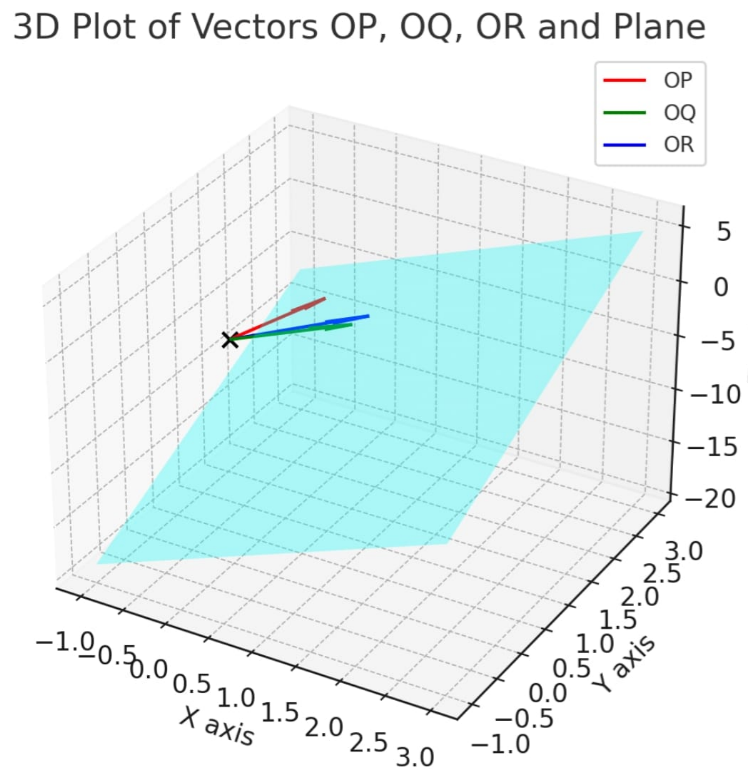
\includegraphics[height=0.5\textheight, keepaspectratio]{fig4.13.105}
    \label{figure_1}
\end{figure}
 
\end{document}